\section{LQG Control Design}
We decided to implement the \emph{LQR} controller as representative of state-feedback schemes. Unfortunately, because of noise in the current sensor, a Kalman Filter was needed. In fact a simple low pass filter on the current feedback was not adequate enough, since it would make the system too slow. The Kalman Filter has been fed with the reference voltage, current flowing in the motor and the cart position.\\

Remember that LQR solves the optimal problem:
\begin{equation}
min J = \int_0^{\infty} x^T Q x + u^T R u dt
\end{equation}
which gives an optimal solution in the form of feedback control:
\begin{equation}
u=-Kx
\end{equation}
First we decided to try an LQG design with an integrator, by adding an extra state: 
\begin{equation}
\dot{e} = -x+r
\end{equation}
But this gave unacceptable performances. To have good performances, by simulations we needed to have the state matrix weight $Q$ with very large eigenvalues, greater than $10^2$. Because of that the feedback gain $K$ was very large, and the control input $u$ saturated the motor, and made the system unstable. The integrator problem can be explained by root locus techniques, as explained in the Positive Zeros Control section. \\ \\
To solve this problem we removed the integrator and added a feedfoward gain on the reference:
\begin{equation}
u=-K_{x} x+ K_{r} r
\end{equation}
Where $K_{r}$ is:
\begin{equation}
K_{r} = \frac{1}{C(-(A-BK))^{-1}B}
\end{equation}
With $C$ selecting the appropriate output, in this case $x_1$, thus $C=\begin{bmatrix}0 & 100 & 0\end{bmatrix}$. This $K_r$ makes sure the system has unitary gain. \\
The weight matrix was selected in order to let $x_1 \to 0$ quickly with acceptable performances. After some iterations the matrices $Q$ and $R$ were chosen as:
\begin{equation}
Q = \begin{bmatrix}
0 & 0 & 0 \\ 0 & 0.5 & 0 \\ 0 & 0 &0 
\end{bmatrix}
\qquad
R=1
\end{equation}

Moreover, the LTR procedure was not considered since there is no noise in the control input channel.
Results are shown below for $K_l$ and $K_h$. Notice the static error, induced by the fact that the non-linearities of the motor were not considered (such as the dead-zone, which changes the gain of the system).\\

  \begin{figure}[!tbh]
  \centering
  \subfloat[LQG $K_l$]{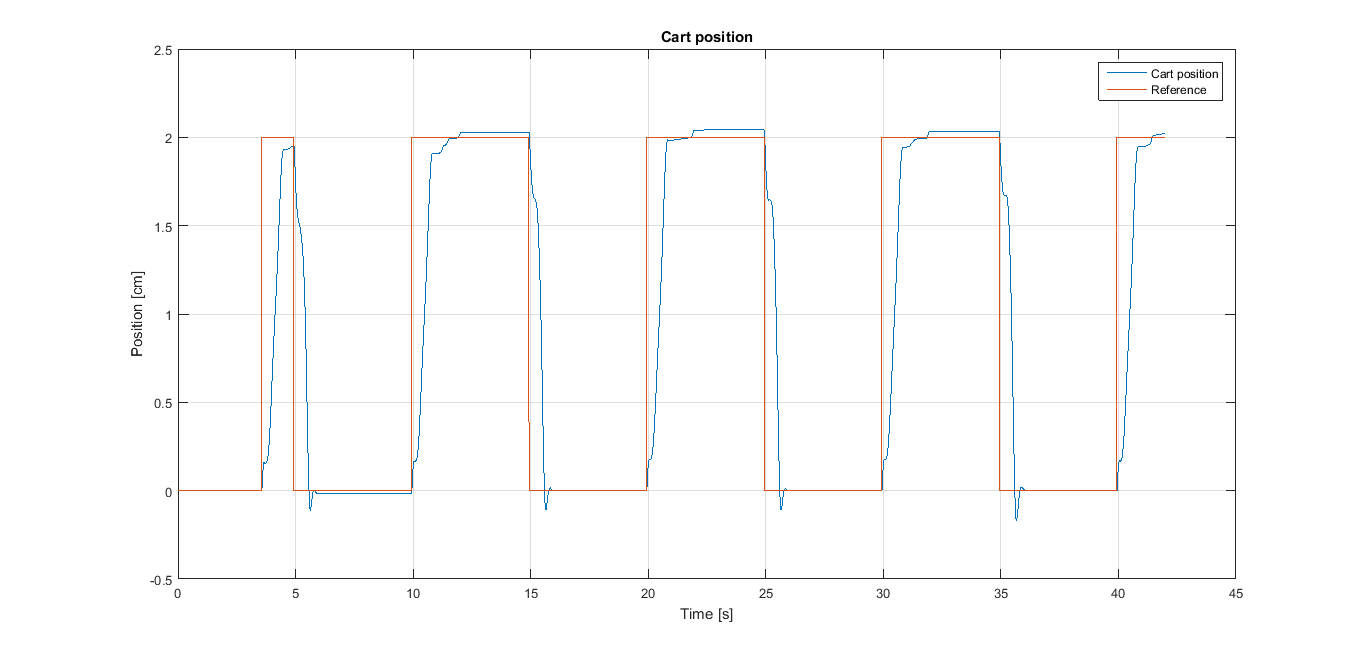
\includegraphics[width=0.6\textwidth]{img/lqg_1dof_klow.png}}
  \hfill
  \subfloat[LQG $K_h$]{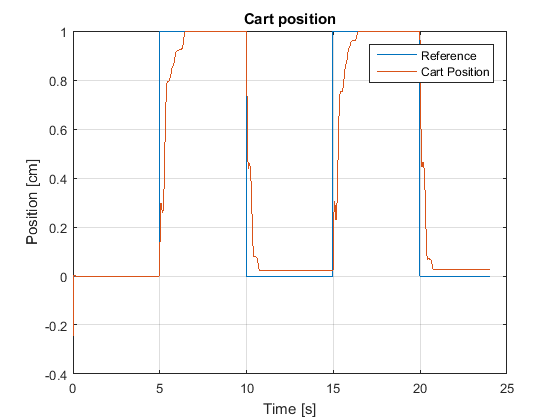
\includegraphics[width=0.4\textwidth]{img/lqg_1dof_khigh.png}}
  \caption{On the left: plot of the cart position with LQG control and $K_l$. On the right plot of the cart position with $K_h$.}
    \label{fig:lqg1dof}
\end{figure}